\section{Implementation}
\label{sec:implementation}

The implementation follows the same design principle that underlies
GradDFT\cite{GradDFT}: fixed electronic-structure inputs are separated
from the differentiable program that evaluates energies,
self-consistent fields, response matrices, and losses.
For GradTDDFT the distinction is extended to excited-state response.
Molecular preprocessing constructs the fixed numerical representation
of a calculation, while the differentiable core operates on density
matrices, orbital rotations, local density variables, and neural
functional parameters.

% ======================================================================
\subsection{Molecular State and Fixed Data}

A GradTDDFT calculation begins from the same physical inputs as a
conventional KS or TDDFT calculation: nuclear charges and coordinates,
charge, spin, basis set, exchange-correlation functional, quadrature
grid, and convergence settings. PySCF is used to construct the
molecule, basis metadata, quadrature grid, AO values on grid points,
one-electron integrals, and electron-repulsion data. These quantities
are then treated as fixed arrays during the differentiable SCF and
response calculation. This boundary keeps the integral and grid
generation path aligned with PySCF reference calculations while
placing the density-dependent part of the method inside JAX.

The fixed molecular state contains the overlap matrix $S$, core
Hamiltonian $h$, grid weights, AO values and derivatives, nuclear
repulsion energy, and the selected representation of the two-electron
integrals. GradTDDFT supports dense electron-repulsion tensors,
density-fitted contractions, and direct J/K construction. The choice
of J/K backend changes how Coulomb and exchange contractions are
formed, but not the mathematical objects passed to the SCF or TDDFT
layers.

% ======================================================================
\subsection{Differentiable SCF and TDDFT Execution}

After molecular preprocessing, the SCF layer is evaluated entirely as
a differentiable fixed-point computation. For a density matrix $P$,
the implementation assembles
\begin{equation}
  F[P;\theta]
  =
  h + J[P] + F_{\rm xc}[P;\theta] + F_{\rm nl}[P;\theta],
\end{equation}
where $J[P]$ is the Coulomb contribution, $F_{\rm xc}$ is the
semilocal or neural XC potential, and $F_{\rm nl}$ denotes optional
nonlocal HF and MP2/PT2-channel contributions. The SCF map diagonalizes
the generalized eigenvalue problem, updates occupations and density,
and repeats this operation until the selected convergence criteria are
satisfied. The converged state stores orbitals, orbital energies,
occupations, density matrices, total energies, and diagnostic
residuals needed by both response calculations and training losses.

The differentiable program can be evaluated either through an
explicit finite SCF trace or through an implicit fixed-point
gradient. Both modes use the same molecular state and Fock-building
path. This is important for comparing training objectives: changes in
the gradient treatment should not change the forward SCF solution
used to build the TDDFT response problem.

The TDDFT layer is differentiated in the same operator-first spirit.
For a converged SCF state, the implementation builds matrix actions
for the TDA or full Casida response problem from orbital-energy
differences, Coulomb and exchange contractions, semilocal XC response
actions, and nonlocal neural-channel response terms. During training,
the Davidson solver is used only as the forward numerical procedure
for obtaining the requested low-lying roots. Following the implicit
differentiation formulation for iterative eigensolvers by Lei Wang and
co-workers,\cite{Xie2020DominantEigensolverAD} GradTDDFT uses a
differentiable Davidson mode in which the reverse-mode derivative
is not taken through the Davidson iteration history, but through the
stationarity of the converged Ritz pairs. In practice, the
matrix-vector products used inside the Davidson iterations are
detached from the reverse pass. After convergence, the Ritz
amplitudes are also held fixed and the excitation energy is
reconstructed as a Rayleigh quotient of the current response
operator. Gradients of excitation-energy losses therefore flow
through the response matrix-action builder, the SCF fixed point, and
the neural functional parameters, while avoiding a large
differentiation tape for the iterative eigensolver. Oscillator
strengths and broadened spectra are evaluated from the same forward
roots; their present training path does not include an additional
eigenvector-response derivative beyond this fixed-amplitude
reconstruction. Detailed formulas for the TDA and Casida root-energy
derivatives are given in the Supporting Information.

% ======================================================================
\subsection{Functional Evaluation and Response Core}

The functional interface is organized around a local energy-density
map. For traditional semilocal functionals, the map evaluates a
specified LDA, GGA, or meta-GGA energy density on the grid. For
neural functionals, local density descriptors are combined with
learned coefficient fields that mix semilocal, HF, and optional MP2/PT2
channels. In both cases the scalar XC energy is obtained by numerical
quadrature, and the SCF potential follows from differentiating the
same energy expression with respect to the density variables.

The conventional semilocal energy-density components are evaluated
through the JAX-XC functional library,\cite{JAXXC} with hybrid exact
exchange handled by the nonlocal HF channel. JAX-XC provides a broader
catalogue of Libxc-translated LDA, GGA, meta-GGA, and hybrid functional
routines than the subset used below. For the GradTDDFT implementation
and the calculations in this manuscript, the default validated
functional inputs include:
\begin{itemize}
  \item LDA and local-correlation components: LDA exchange,
    Perdew--Wang correlation, Vosko--Wilk--Nusair correlation, and
    the VWN-RPA variant.
  \item GGA components: Becke 88 exchange, PBE exchange, the
    range-separated PBE exchange component, LYP correlation, and PBE
    correlation.
  \item Composite local and semilocal specifications: LDA, SVWN,
    SVWN-RPA, PBE, and the local semilocal part of LC-WPBE.
  \item Global and screened hybrid specifications: PBE0/PBEH, B3LYP,
    BHandHLYP, HSE03, and HSE06. Their semilocal terms are routed
    through JAX-XC, while the HF fraction is assembled by the exact
    exchange contraction path.
\end{itemize}
Additional installed JAX-XC names, including further GGA, meta-GGA,
and hybrid components, can be routed as optional channels after
validation for the selected SCF and TDDFT response path. They are not
part of the default validated set used for the calculations described
here.

The TDDFT response layer reuses the converged SCF state and constructs
the TDA or full Casida matrices from orbital-energy differences,
Coulomb and exchange response contractions, and the XC kernel. For
semilocal response, the local kernel is the Hessian of the same
energy-density map used for the SCF potential. This gives a single
source for $E_{\rm xc}$, $v_{\rm xc}$, and $f_{\rm xc}$ rather than
three separately implemented formulas. The corresponding data flow for
traditional functionals is summarized in
Figure~\ref{fig:traditional-response-core}.

\begin{figure}
  \centering
  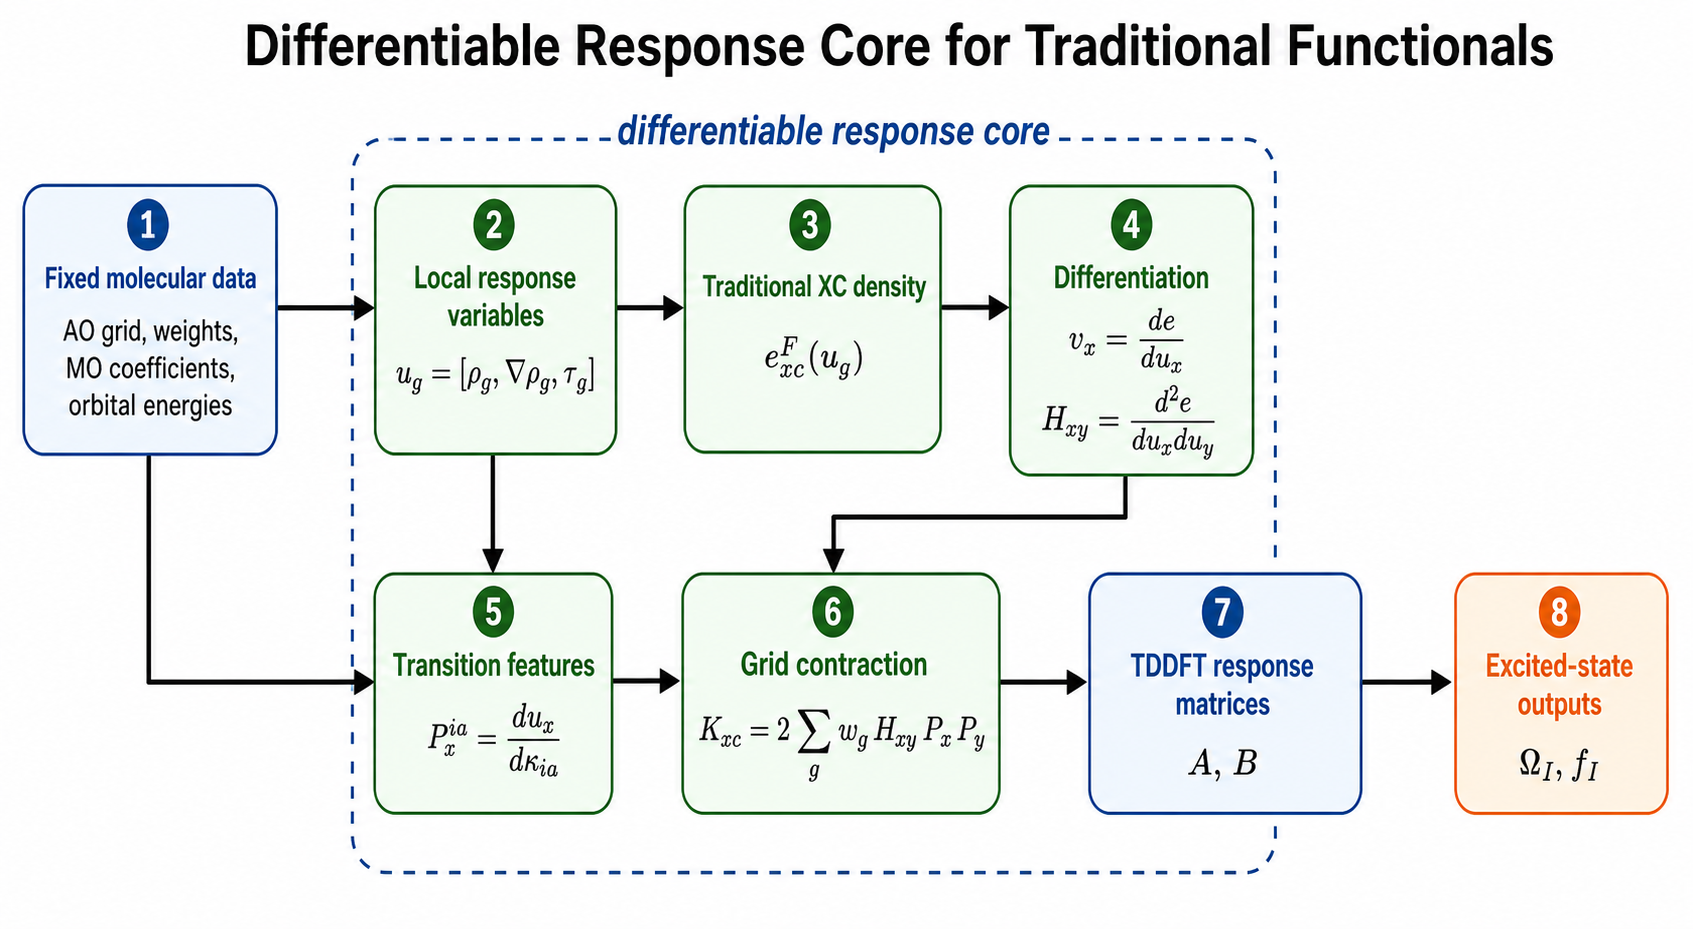
\includegraphics[width=\linewidth]{figures/figure3-traditional-response-core-gpt-image2.png}
  \caption{Differentiable response-core construction for traditional
    semilocal functionals. Fixed molecular data define local density
    variables and transition response features, while differentiation
    of the XC energy density supplies the potential and local Hessian
    used to assemble TDDFT response matrices.}
  \label{fig:traditional-response-core}
\end{figure}

For the neural HF channel, the response binding converts the learned
local exchange field into a density-weighted scalar exchange fraction
and inserts it into the same nonlocal exact-exchange contractions used
by hybrid TDDFT. For the neural MP2/PT2 channel, the response solver
first obtains the TDA or Casida singles roots and then applies a
state-specific CIS(D)-type second-order correction scaled by the
learned PT2 coefficient. This is the calculation path used for the
excited-state tests described in Section~\ref{sec:results}.

% ======================================================================
\subsection{Training and Observable Evaluation}

The final computational graph maps neural parameters to scalar losses.
Starting from the fixed molecular state, GradTDDFT performs SCF,
constructs the response matrices, solves the TDA or full TDDFT
eigenvalue problem, and evaluates observables such as excitation
energies, oscillator strengths, transition dipoles, state-ordering
metrics. Figure~\ref{fig:computation-flow}
summarizes this end-to-end path.

\begin{figure}
  \centering
  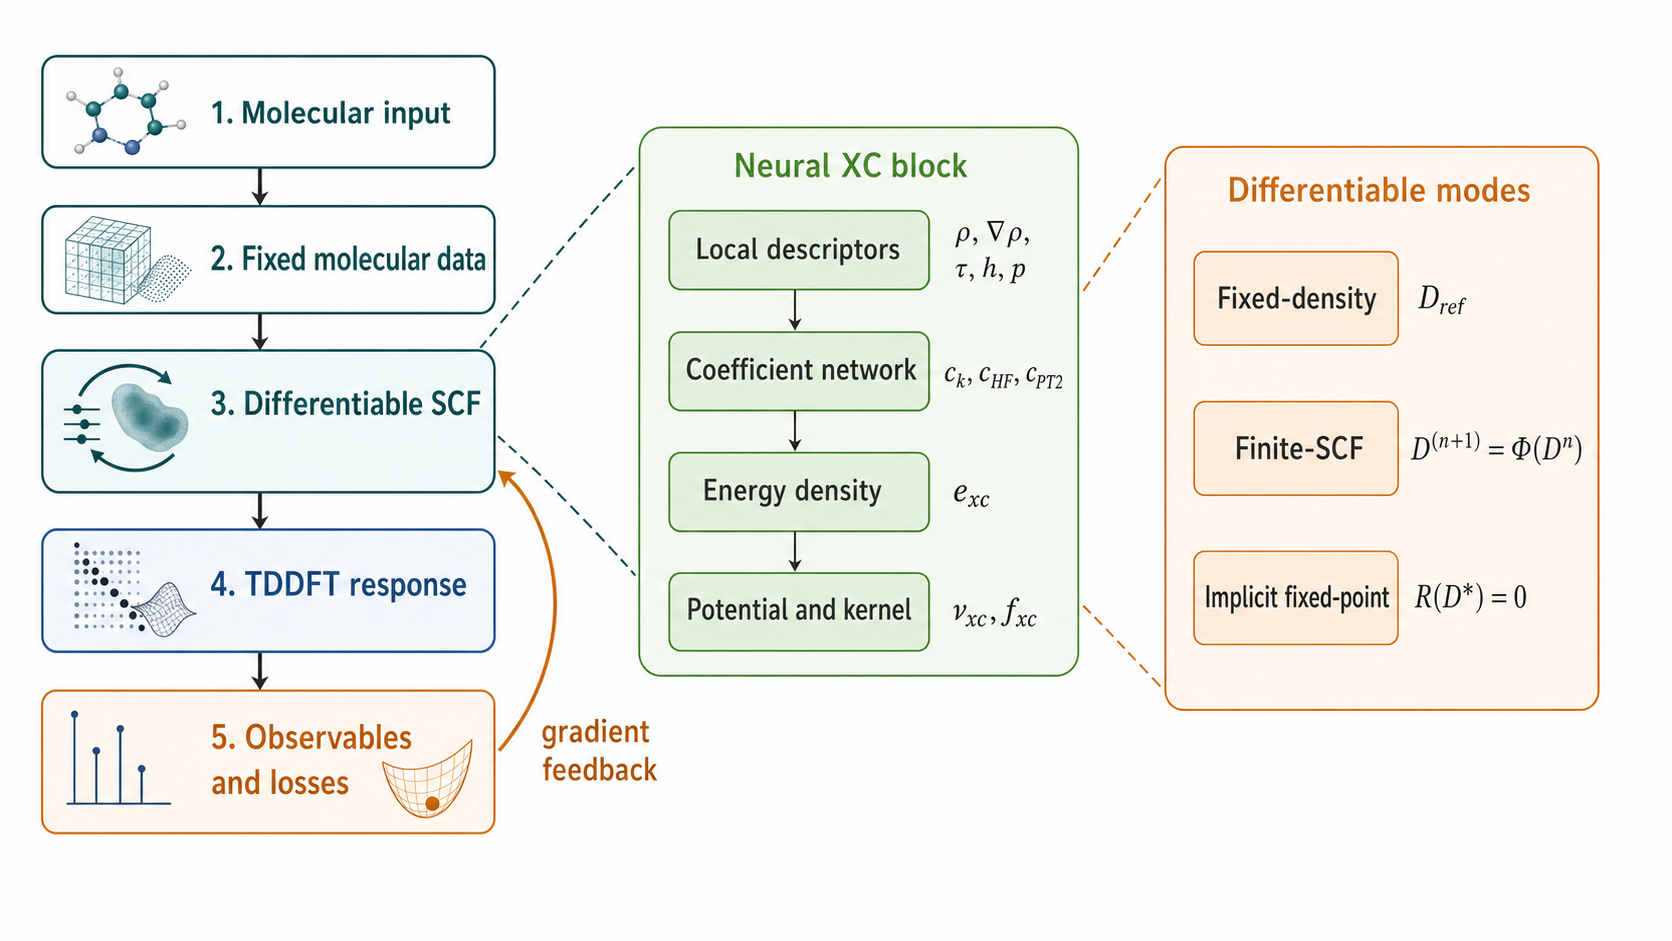
\includegraphics[width=\linewidth]{figures/figure2-computation-flow-sphnet-style-gpt-image2.png}
  \caption{End-to-end computation flow for differentiable
    ground-state and excited-state training.
    Fixed molecular data are passed through SCF and TDDFT response
    construction to produce observables and scalar losses whose
    gradients propagate back to the neural functional parameters.}
  \label{fig:computation-flow}
\end{figure}

Loss terms can target ground-state energies, excitation energies,
oscillator strengths, or state-ordering diagnostics. The current
training protocol optimizes ground-state and excited-state objectives
in separate runs.
Each calculation records the SCF convergence
status, response solver, excited-state treatment, backend, seed, and reference
labels. These records separate numerical failures from functional
errors.

% ======================================================================
\subsection{Verification}

Verification uses matched PySCF calculations and gradient audits.
Runs with traditional functionals compare SCF energies, orbital
energies, TDA and full TDDFT excitation energies, oscillator
strengths, transition dipoles, and response-matrix components against
PySCF references. The matched settings include geometry, basis, grid,
functional, and spin treatment. These tests establish that the
differentiable path reproduces the reference TDDFT calculation before
neural parameters are introduced.

Differentiability audits evaluate representative scalar losses through
the full SCF, response, and observable graph. The audits check finite
values, finite gradients, and nonzero parameter sensitivity. They are
run for explicit finite-SCF differentiation and implicit fixed-point
gradients, together with implicit TDDFT root differentiation, ensuring
that the implementation can support the training paradigms described
in Section~\ref{sec:theory}.
